\documentclass[a4paper,10pt]{article}
\usepackage{graphicx}
\usepackage{subfigure}
\usepackage[pdfborder={0 0 0}]{hyperref}
\title{ Student Project 2017 \\ CalTech101 Image Classification}
\author{David Schulte, Hannes Martinke, Martin Zettwitz}

\begin{document}
\maketitle

\section{Introduction}
The classification of arbitrary pictures is an actual very hard task for image analysts, because the machine learning methods are difficult to use with the high number of pixel features in an image.
The task of the project is to classify the \emph{CalTech 101} dataset by using different feature selection and classifying approaches. 
The dataset contains images of 101 different categories. We had to achieve an accuracy of 10~\% with a 10-Fold cross validation.

\paragraph{Programming Environment}
Our classification approach is implemented in C++ with the use of \emph{Opencv} and \emph{dlib}.
\emph{Opencv} and \emph{dlib} are open source libraries for computer vision and machine learning tasks. 
Our first approaches were an implementation in \emph{Opencv}, because of some missing algorithm for the classification step in the library, we added the \emph{dlib} to combine both libraries.
The workflow of our procedure consists of the following four steps: preprocessing, features generation, training, validation.
The steps will be explained in the next sections.

\section{Preprocessing}
\label{sec:preprocessing}
Several images in the \emph{CalTech 101} dataset exist in different resolutions. 
This results in different lengths of the feature vectors within the feature generation.
To avoid this problem we resized each image in the data set to 64x64, respectively 128x128 and 256x256.
An additional reason for the resizing is the computation time of the feature generator and the training itself. 
We tried to get a good trade-off between accuracy and computation time.
\begin{figure}[ht]
\centering
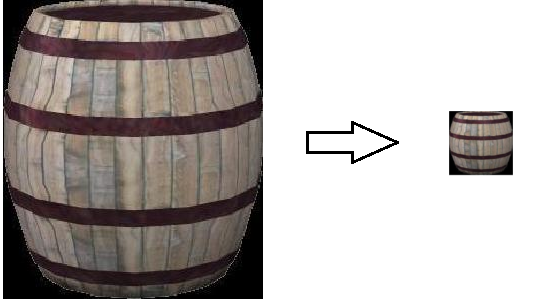
\includegraphics[scale=0.5]{images/preprocessing.png}
\caption{Illustration of the image re-sampling with an example image of a barrel.}
\label{fig:resize}
\end{figure}

\section{Features}
\subsection{Feature Generation}

We used the Histogram-of-Oriented-Gradients~(HOG) as described in ~\cite{McC86}~\cite{DT05}
and Local-Binary-Pattern~(LBP) as described in~\cite{OPH94}
feature descriptors as they are powerful techniques to describe images independent of the lighting conditions.
These techniques use two different approaches to describe features. In general HOG uses a shape description using edges were LBP uses information based on the texture.

\paragraph{HOG} 
The Image is split into connected regions called cells. The edges (defined by gradients) are assigned into different bins (uniformly distributed directions).
The implementation from dlib accepts 3 additonal parameters besides the input image.
Cellsize and 2 parameters for padding rows/columns. The first parameter sets the height/width of the square cells. 
Since we did not use filtering on those features, the padding stayed 1. During the process we lose rows/colums at the borders due to the filtering nature of the hog generation.

The length of the final feature vector for each image is therefore (image.columns / cellsize - 2)  * (image.rows / cellsize - 2) * 31.
We tested the cell size with 8, 16 and 32.
The original image and two example images with the different parameter setups are shown in figure \ref{fig:hog}.
It is to note that there is no visivle difference between image size 256 x 256 and a cellsize of 16 and an image size of 128 x 128 and a cellsize of 8.

\begin{figure} [htb] 
	\centering 
	\subfigure[original image]{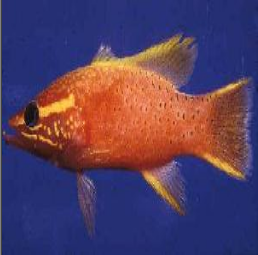
\includegraphics[width=3cm, height= 3cm]{images/hog/256_256_original_fish}}  
	\subfigure[HOG image cell size 8]{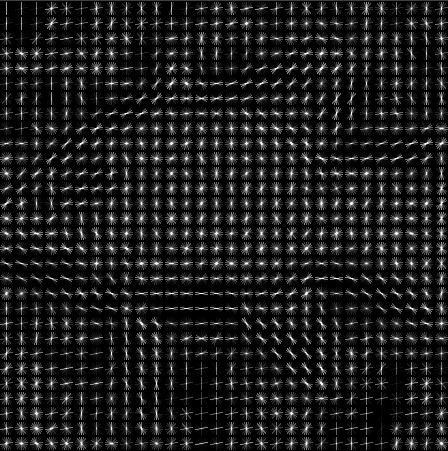
\includegraphics[width=3cm, height= 3cm]{images/hog/256_256_8}}  
	\subfigure[HOG image cell size 16]{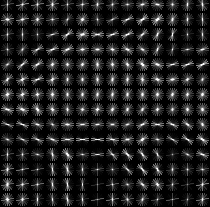
\includegraphics[width=3cm, height= 3cm]{images/hog/256_256_16}}  
	\caption{Illustration of the HOG feature descriptor. Figure a shows the original image with size 256x256 and image b and c display the HOG features.} 
	\label{fig:hog} 
\end{figure}

\paragraph{LBP}
In the dlib implementation the image is overlayed with densely tiled windows that have a width and height of the cellsize. The windows do not overlap and the cellsize should be chosen so that the windows cover the whole image. The LBP histograms are generated in those windows. 
The resultig feature vector has the length of (image.columns / cellsize)  * (image.rows / cellsize ) * 59.

We used for the cell size 8 and 64 for experimenting.

\subsection{Feature Reduction}

The calculated features can be reduced by using principle component analysis(PCA) or other techniques.
In our approach a feature reduction is served by re-sampling the images in the preprocessing step (recall \autoref{sec:preprocessing}).
With the limitation of the pixel matrix and the use of HOG/LBP features, the length of the feature vector is equalized for each sample.

For example, a single run with LBP features and SVM as a classifier with an image size of 64 x 64 and cellsize of 8 took 108 minutes on a modern quadcore cpu, even with mutiprocessing.
\section{Classifiers}

After generating the feature vectors for each sample, the samples of each class must be trained, followed by testing to evaluate the accuracy of the whole classification approach. 
Therefore we implemented two different classifiers. 

\paragraph{AdaBoost}
Adaptive Boosting \emph{INSERT PAPER Fre95} is machine learning approach, that is based on so called \textit{weak classifiers} that will form a \textit{strong classifier}. Each weak classifier is assigned to randomly generated feature, its prediction is just slightly better than random guessing. The power of the technique is done by combining the best $n$ weak classifiers to a strong classifier as a powerful descriptor. The weak classifiers are trained by supervised learning where each weak classifier predicts the samples. Based on that prediction the error rate is assigned to the individual weak classifier. Additionally each sample is weighted by its significance (error rate of the best weak classifier) to emphasize unseen and hard to predict training data. Based on that significance weight and the error rate of a weak classifier, each weak classifier that is combined to the strong one is weighted, too.
\paragraph{SVM}
A Support-Vector-Machine basically tries to define a hyperplane to distinguish between classes in datasets. Therefore support-vectors are created, that maximizes the distance between the closest points of (two) classes. To separate between non-linear datasets, the feature space is mapped onto an higher dimensional space, using a kernel, where a linear separation is possible. Mapped back onto the original feature space one obtains the hyperplane. This way even initial high dimensional datasets can be distinguished. To reduce the computational effort one uses Mercer's theorem, that only implicitly computes the data in the higher dimension, but instead uses a kernel function. Well used kernels are polynomial kernels and radial-base-function kernels like Gaussian. We used a Nu-SVM with parameter $Nu$ as constrain for the hyperplane in a range of $[0,1]$. We tested several values by iteratively increasing $Nu$ until the classification error was minimized with a $Nu$-value of $0.00511$ 

\section{Training and Validation}
To train and validate our approach we used a 10-fold cross validation. 
This method divides the data set in 10 subsets of equal size. Each fold contains the same amount of images from each class, were the target class is labeled as positive sample and the other classes as negative samples. 9 folds will be trained and the last one is for testing of the classifier.
This is an iterative process and will be performed using permutation until each fold was tested.
\paragraph{Validated Images}
To observe the process, we counted the number of predictions and assigned the positive predictions to the predicted class.
To prepare a balanced test we detect the smallest number of samples in a class and took the same number of samples of the other classes in the training and testing. 
Consequently we preserve that the same number of images will be tested and trained.
\section{Results}
Our best result was 46.69 \% of correct predicitons.
We achieved this result with an image size of 64 x 64 , HOG features with cellsize 8 and a SVM classifier with a nu of 0.004652.
Similar results were achieved with an image size of 128 x 128 and a cellsize of 16, which was expected, since the resulting feature images were really similar.
Since the SVM classifier yields better results and was faster (e.g. when SVM achieved 46\% in 6 minutes, AdaBoost achieved 38\% and took 9 minutes) we focused our testing runs on SVM.
Boost seemed to have a problem with overfitting, due to time limitations we didn´t inspect this issue further when we had an alternative at hand.
LBP features turned out to be a weak features in the context of the CalTech101 Challenge and the used classifiers.
The best prediction rate we achieved with LBP was 31.28\%, suprisingly with image size of 64 x 64 and a cellsize of 64 in only 2 1/2 minutes. So every feature vector for an image was only 59 float entries long. Even runs with a cellsize of 8, which yielded in a feature vector per image of length 3776 only achieved 29\% and took 108 minutes.
We conclude that LBP got all the necessary information even on small image sizes / big cellsizes. 

Our strongest classes where anchor and revolver, with around 80\% of correct predictions. 
The images in this classes have strong and mostly clear edges, which is exactly the information we wanted to extract with the HOG features. 
Also the objects in the images had often the same orientation, which would have been a weak point with this feature.
The weakest class was faces\_easy, which is understandable since there is a class faces, too. Class Garfiled was precited correct only 15\% of the time. Even though the edges are clear on the images, the orienation and his posture changes, which gives very different feature vectors for the same class.

You can see our results in a confusion matrix in the appendix (confMat.xlsx)

\bibliography{citaviFiles}
\bibliographystyle{plain}
\end{document}

\grid
\grid
